\documentclass[12pt]{article}
\usepackage[utf8]{inputenc}
\usepackage{graphicx}
\usepackage{amsmath}
\usepackage{booktabs}
\usepackage{geometry}
\usepackage{float}
\usepackage{siunitx}

\geometry{a4paper, margin=1in}
\title{Lashing Calculation Report}
\author{Lashing Calculator}
\date{\today}

\begin{document}
\maketitle

\section{Input Parameters}

\subsection{Load Specifications}
\begin{table}[H]
\centering
\begin{tabular}{ll}
\toprule
Parameter & Value \\
\midrule
Length (X) & \SI{3.0}{m} \\
Width (Y) & \SI{23.0}{m} \\
Height (Z) & \SI{2.7}{m} \\
Mass & \SI{160.0}{tonnes} \\
\bottomrule
\end{tabular}
\end{table}

\subsection{Environmental Conditions}
\begin{table}[H]
\centering
\begin{tabular}{ll}
\toprule
Parameter & Value \\
\midrule
Slope & \SI{3.0}{\degree} \\
Wind Force & Beaufort 0 \\
Friction Coefficient & 0.2 \\
\bottomrule
\end{tabular}
\end{table}

\subsection{Lashing Configurations}
\begin{table}[H]
\centering
\begin{tabular}{cccccc}
\toprule
Lashing & $\alpha$ & $\beta$ & Breaking Strength & Side \\
\midrule
1 & \SI{4.0}{\degree} & \SI{4.0}{\degree} & \SI{4.0}{Tonnes} & F \\
2 & \SI{4.0}{\degree} & \SI{5.0}{\degree} & \SI{5.0}{Tonnes} & R \\
\bottomrule
\end{tabular}
\end{table}

\section{Calculation Results}

\subsection{Transverse Sliding Analysis}
\begin{verbatim}
Transverse sliding!! Check lashing!
You need 27 more lashing on rear

\end{verbatim}

\subsection{Longitudinal Sliding Analysis}
\begin{verbatim}
Longtidunal sliding occurs.
You need 62 more lashing on front or back

\end{verbatim}

\section{Lashing Configuration Diagram}
\begin{figure}[H]
\centering
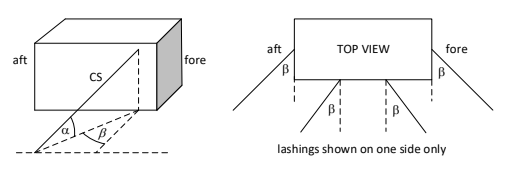
\includegraphics[width=0.8\textwidth]{pics/lashingPic.png}
\caption{Lashing Configuration}
\end{figure}

\end{document}